\chapter{Wrap-up}
This chapter connects the dots that are the many different observations and conclusions made in previous chapters, describing both what has been done and what could still be done and is meant to close the arc between my \acs{CESM} experiments (\chapref{chap:cesm-runs}) and theoretical studies (\chapref{chap:analysis}).

\secref{sec:outro-summary} gives a summary of the main results of my thesis, while \secref{sec:outro-outlook} discusses some open questions and how they could be tackled in future work.

\section{What Have We Learned?}
\label{sec:outro-summary}
The following sections describe the observations I have made when lowering the western boundary layer viscosity at the equator in \acs{CESM} experiments with low (\grid{x3}) and intermediate (\grid{x1}) resolution (\chapref{chap:cesm-runs}), along with my \q{best guess} on how to interpret these results, taking into account the theoretical findings from \chapref{chap:analysis}.

A particular focus lies on the generation of numerical noise (\secref{sec:outro-noise}), cross-equatorial flow in the Atlantic (\secref{sec:outro-amoc}), and the \ac{ITF} (\secref{sec:outro-itf}).

\subsection{Numerical Noise}
\label{sec:outro-noise}
The main result of \secref{sec:cesm-noise} is that, while an intact boundary layer with low grid scale Reynolds numbers is critical for numerical noise suppression in the equatorial regions\sidenote[-2]{Which I hypothesized to be the case because information always travels \emph{westward} in the ocean, hence noise created in the interior basin can not be dissipated without a western boundary layer.}, the smoothed velocity field is still a decent representation of the actual dynamics.

Noise is mostly created on grid scale and preferably in zonal direction, which is also observed in my shallow-water model. This is probably due to the fact that 1) meridional grid spacings are smaller than those in zonal direction close to the equator, and that 2) velocity shears are dominantly in zonal direction (due to the sharp western boundary layer). 

The total amount of generated noise under viscosity reduction seems to depend critically on the given grid spacing --- much less noise is observed in \grid{x1} or the high-resolution shallow-water experiments, even when grid scale Reynolds numbers are high.

\subsection{The \acl{AMOC}}
\label{sec:outro-amoc}
The total transport carried by the \ac{AMOC} only depends weakly on viscosity. When only accounting for contours of the vertical \ac{AMOC} stream function that penetrate far into the opposite hemisphere, the transport changes by a maximum of \SI{-1.5}{\sv} (for \run{x3_nomunk}, where the Munk layer viscosity has been globally reduced to the much lower background value), while integrating directly over the velocity at the equator yields a maximum change of about \SI{-1.2}{\sv} (again, for \run{x3_nomunk}). This is less than anticipated intuitively, considering that, without friction, the required transformation of \ac{PV} to enable cross-equatorial flow is impossible. However, it is shown that the efficiency of \ac{PV} transformation inside a Munk boundary layer is independent of viscosity to a leading order (\secref{sec:killworth}).

On the other hand, I \emph{did} observe a clear correlation between viscosity and cross-equatorial transport, where lower viscosities always led to a decreased transport, and vice versa. In order to understand this behavior, I have tried to produce a similar response in an equatorial shallow-water model that is forced by a constant buoyancy forcing and uniform \q{upwelling} across the domain. After running several simulations in different scenarios (\secref{sec:equatorial-shallow-water}), I was not able to reproduce the observed response in this simple model\sidenote[0]{Instead, transports were either independent of viscosity, or increased for smaller viscosities (if the boundary layer was under-resolved).}. I thus conclude that the response of the ocean in \ac{CESM} depends on effects that were not included in my model (some possible candidates are discussed in \secref{sec:outro-moc-viscosity}).

Looking at the flow field around the equator in the Atlantic in \ac{CESM}, I noticed deep, zonal equatorial jets (similar to those described in \cite{greatbatch-jets}) that emerge along the equator and extend all the way to the eastern boundary, where it seems like some boundary layer interactions took place. In \ac{CESM} experiments with extreme viscosity modifications, a roughly equal amount of water crosses the equator in the eastern and western parts of the basin. \emph{The structure and efficiency of the western boundary thus indeed seems to be affected heavily by strong viscosity modifications.}

\subsection{The \acl{ITF}}
\label{sec:outro-itf}
The total transport crossing the \ac{ITF} shows roughly the same dependence on viscosity as the \ac{AMOC}, with maximum changes of about \SI{-2}{\sv} in \grid{x3}, and \SI{-0.5}{\sv} in \grid{x1}.

On top of these small modifications of the total transport (which are expected to be small considering Munk layer theory as in \secref{sec:killworth}), dramatic changes of the composition of the \ac{ITF} are observed in the \grid{x3} experiments\sidenote[-2]{\grid{x1} experiments seem to be largely unaffected because of a very different geometry around the Indonesian islands.}. The \ac{BSF} suggests that, for extreme viscosity modifications, about half of the total \ac{ITF} originates in the southern hemisphere, versus a purely northern source when using default viscosity parameters. This is reinforced by the salinity profile of this region, which shows a considerably saltier \ac{ITF} for low viscosities, which also hints towards a southern source.

In \secref{sec:island-rule}, I have reviewed Godfrey's Island Rule. Since the Island Rule predicts an \ac{ITF} that only depends on the atmospheric forcing and geometry, the observed dependency of the transport on viscosity seems like a contradiction. An extension of the Island Rule with friction (from \cite{wajsowicz}) predicts a \emph{weaker} transport for \emph{higher} viscosities, \ie the opposite of what is observed in \ac{CESM}. It thus seems like the Island Rule, while it delivers a good first approximation, is indeed not strictly valid at the equator.

After all, the processes that determine the source of the \ac{ITF} are still unclear. Some additional possibilities are discussed in \secref{sec:outro-itf-origin}.

\section{Open Questions}
\label{sec:outro-outlook}
The following sections are meant to point out some loose ends in this study, where future work would be necessary to get a clearer understanding, and presents some further ideas that fell out of the scope of this thesis.

In particular, there are two major open questions, one concerning the total strength of the overturning (\secref{sec:outro-moc-viscosity}), and one concerning the \ac{ITF} (\secref{sec:outro-itf-origin}).

\subsection{How is the overturning modified when changing viscosity?}
\label{sec:outro-moc-viscosity}
Since my shallow-water model could not reproduce \ac{CESM}'s dependence of the overturning on viscosity, it is still unclear \emph{how} the total cross-equatorial transport can be modified by changing viscosity, even though theory predicts that it should be constant to a leading order (\secref{sec:killworth}). Apparently, this response is created by an effect that was not modeled in the shallow-water experiments. Some likely candidates are:
%
\begin{enum}
	\item boundary topography, which modifies the balance between friction and Coriolis force if the boundary layer is not strictly meridional, and bottom topography (see \eg \cite{nofbc2} and \cite{swaters});
	\item interactions between multiple layers, as discussed \eg in \cite{nofbc1}, or the effect of a vanishing layer height (\cf \eqref{eq:munk-friction-balance});
	\item additional forcing by the wind; and
	\item a feedback between the forcing of the model and the amount of equator-crossing flow.
\end{enum}
%
For starters, an enhanced model could include a realistic geometry of the North Atlantic, and explicitly model both branches of the \ac{AMOC} (northward, shallow and southward, deep). This model should be much closer to reality, and hopefully give a realistic dependence on viscosity\sidenote[-3]{One possibility would be to use a verified \acs{GCM} such as the MIT General Circulation Model (MITgcm), which supports idealized processes and geometries, instead of a self-developed model.}.

Another clue towards the processes in a low-viscosity Atlantic is given by the equatorial jets that are observed in some experiments. These jets are studied and modeled in \cite{kitamura}, and a similar study could reveal their connection to cross-equatorial transport and viscosity.

\subsection{What controls the origin of the \acl{ITF}?}
\label{sec:outro-itf-origin}
The origin of the \ac{ITF} is in fact highly discussed in literature\sidenote{\Eg in \cite{nofind}; \cite{godfreyind}; \cite{lukas}; \cite{gordon}.}, and observations suggest a predominantly northern source. However, none of these studies seems to include the dependence of the \ac{ITF} composition on viscosity. Possible explanations for the observed, sensitive dependence of the \ac{ITF} on viscosity are:
%
\begin{items}
	\item In \cite{nofind}, \citeauthorfull{nofind}%
	\sidefigure{The \ac{ITF} model presented in \cite{nofind}.}[fig:nof-setup]{%
		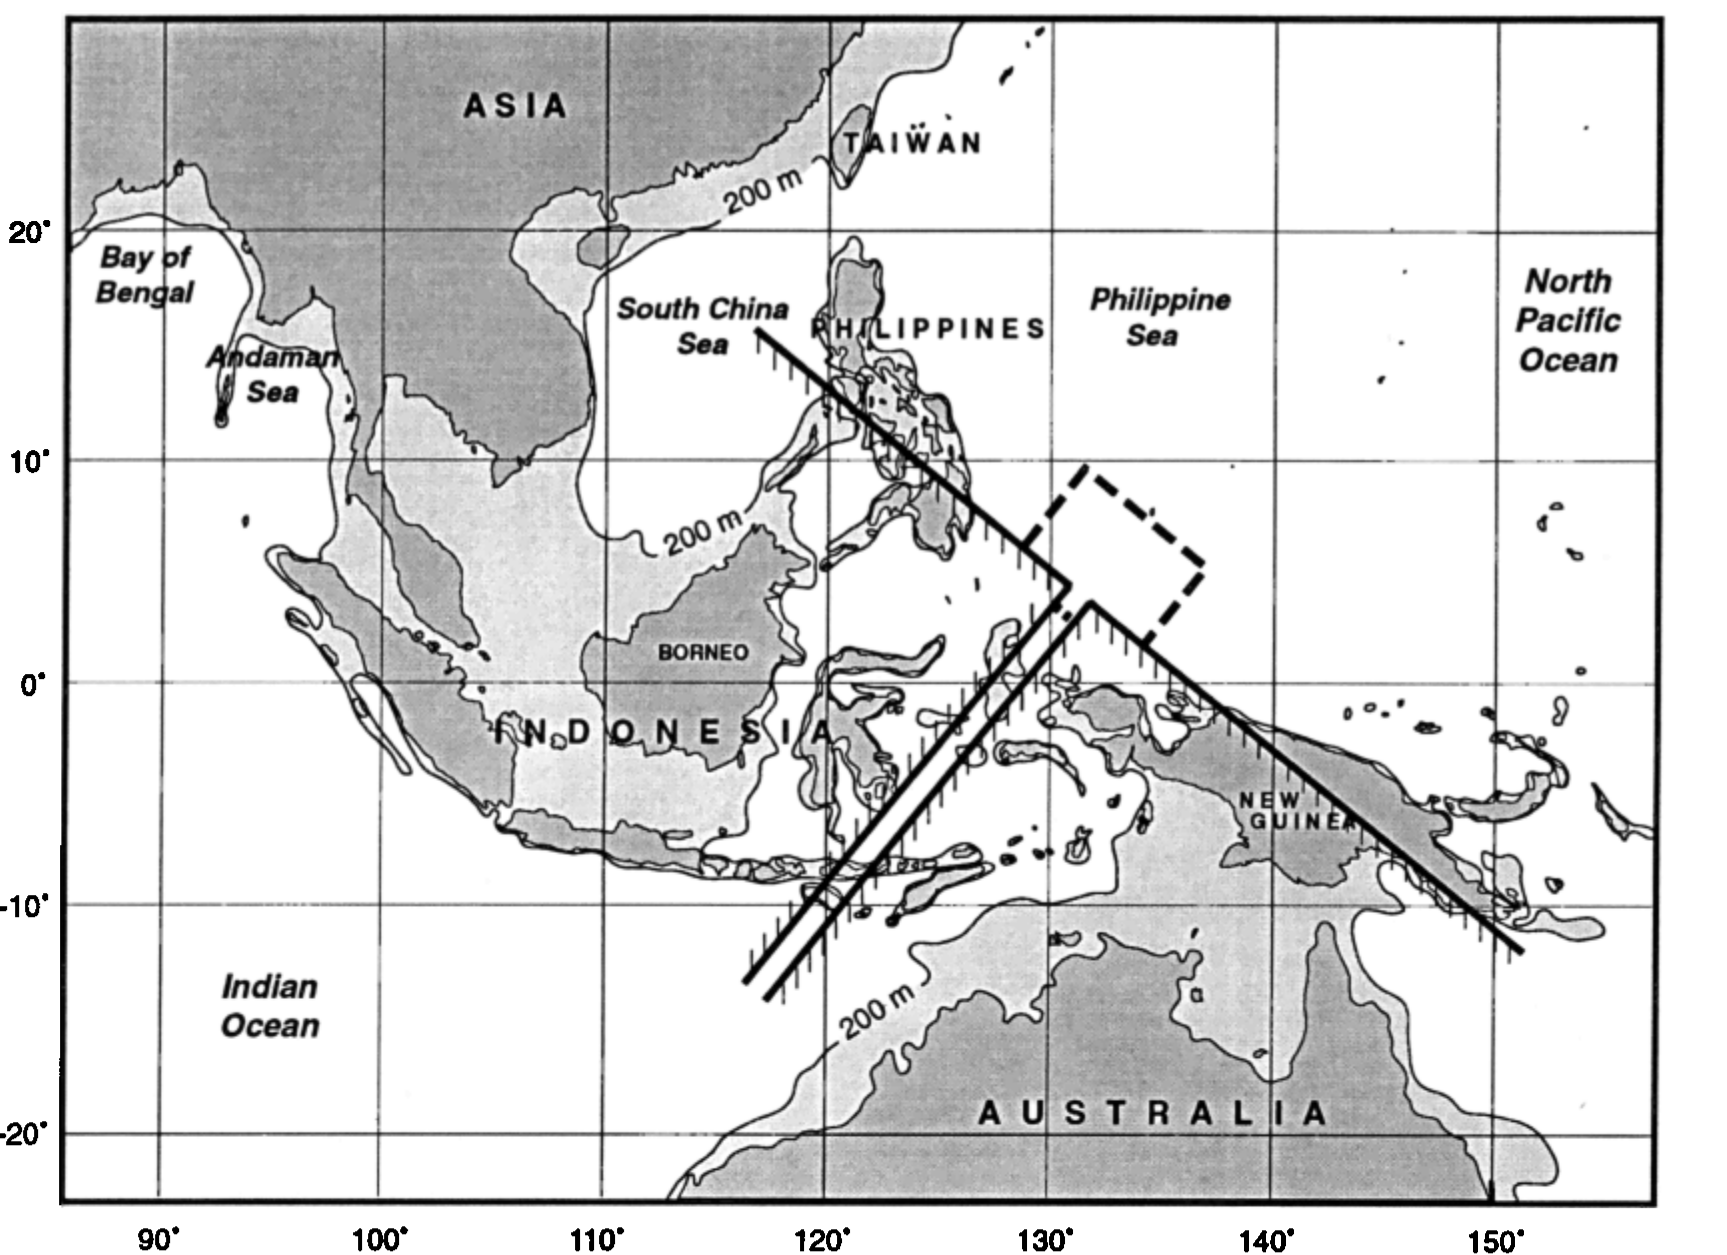
\includegraphics[width=\marginparwidth]{figures/outro/nof}%
	}[1]%
	considers a nonlinear, frictionless model of the \ac{ITF} with an idealized geometry (\figref{fig:nof-setup}). He shows that the determining factor for the origin of the \ac{ITF} in this model is (1) the geometry of the basin and (2) the undisturbed layer heights at certain points of the current system in the \ac{ITF}. While not taking viscosity into account explicitly, these layer heights are certainly influenced by the Munk layer viscosity in this region, which could yield an explanation for the observed behavior.
	\item Since the most direct effect of a reduced viscosity is a lower boundary layer width, it is certainly possible that the ensuing geometrical alteration of the flow path has a direct influence on the solution in the \ac{ITF} region. Even a slightly displaced path may have a large influence eventually, \eg through a spatially dependent wind stress, or the \q{collision} with other currents.
	\item In fact, since the efficiency of the cross-equatorial transport in a western boundary layer \emph{was} found to be influenced dramatically by viscosity in the Atlantic, it seems like the same may be the case here --- flow that fails to dump excess vorticity follows the coast of New Guinea without crossing the equator further than a few Rossby radii of deformation, and then curves back into the southern hemisphere. The flow does not need to form a jet as in the Atlantic, since it never actually crosses the equator in \grid{x3}\sidenote{In contrast to the \grid{x1}-grid, where additional islands require the flow to reach further north in order to curve into the \ac{ITF}, which is thus suppressed.}. However, this interpretation still needs careful testing, \eg in another idealized model with a geometry that is similar to that of the Indonesian islands and New Guinea.
\end{items}
%
%\parabreak
%
\emph{It seems thus, that frictional control of cross-equatorial flow is indeed possible in low-resolution models, and that the chosen model viscosity does have a decisive influence on the flow in the equatorial regions} (though not so much on its total magnitude).